\documentclass[reprint, nofootinbib]{revtex4-2} %preprint: 1
\usepackage[utf8]{inputenc}
\usepackage{graphicx}
\usepackage{float}
% math symbols
\usepackage{amsmath}
\usepackage{xcolor}
\usepackage{amssymb}
\usepackage{amsfonts}
\usepackage{fancyvrb}
% pic
\usepackage{graphicx}
\usepackage{dcolumn}
\usepackage{bm}
\usepackage{hyperref}
\usepackage{mathptmx}
\newcommand{\ud}{\,\mathrm{d}}
\newcommand{\pd}{\partial}
\newcommand{\im}{\mathrm{i}}
\newcommand{\V}[1]{\begin{pmatrix}#1\end{pmatrix}}

\begin{document}
\title{PS3203 Computational Physics: Final 2020}
\author{Hyejin Kim (20185055)}
%\affiliation{GIST college, Gwangju 61005, Republic of Korea}
\email[email: ]{aadeliee@gm.gist.ac.kr}
\date{\today}

\maketitle
\section{The Lorenz equations}
The Lorenz equations is given by
\begin{align*}
	\frac{\ud x}{\ud t} &= \sigma (y-x)\\
	\frac{\ud y}{\ud t} &= rx - y - xz\\
	\frac{\ud x}{\ud t} &= xy - bz
\end{align*}
where $\sigma, r, b$ are constants. This equations shows some chaotic motion.

\begin{figure}[t]
	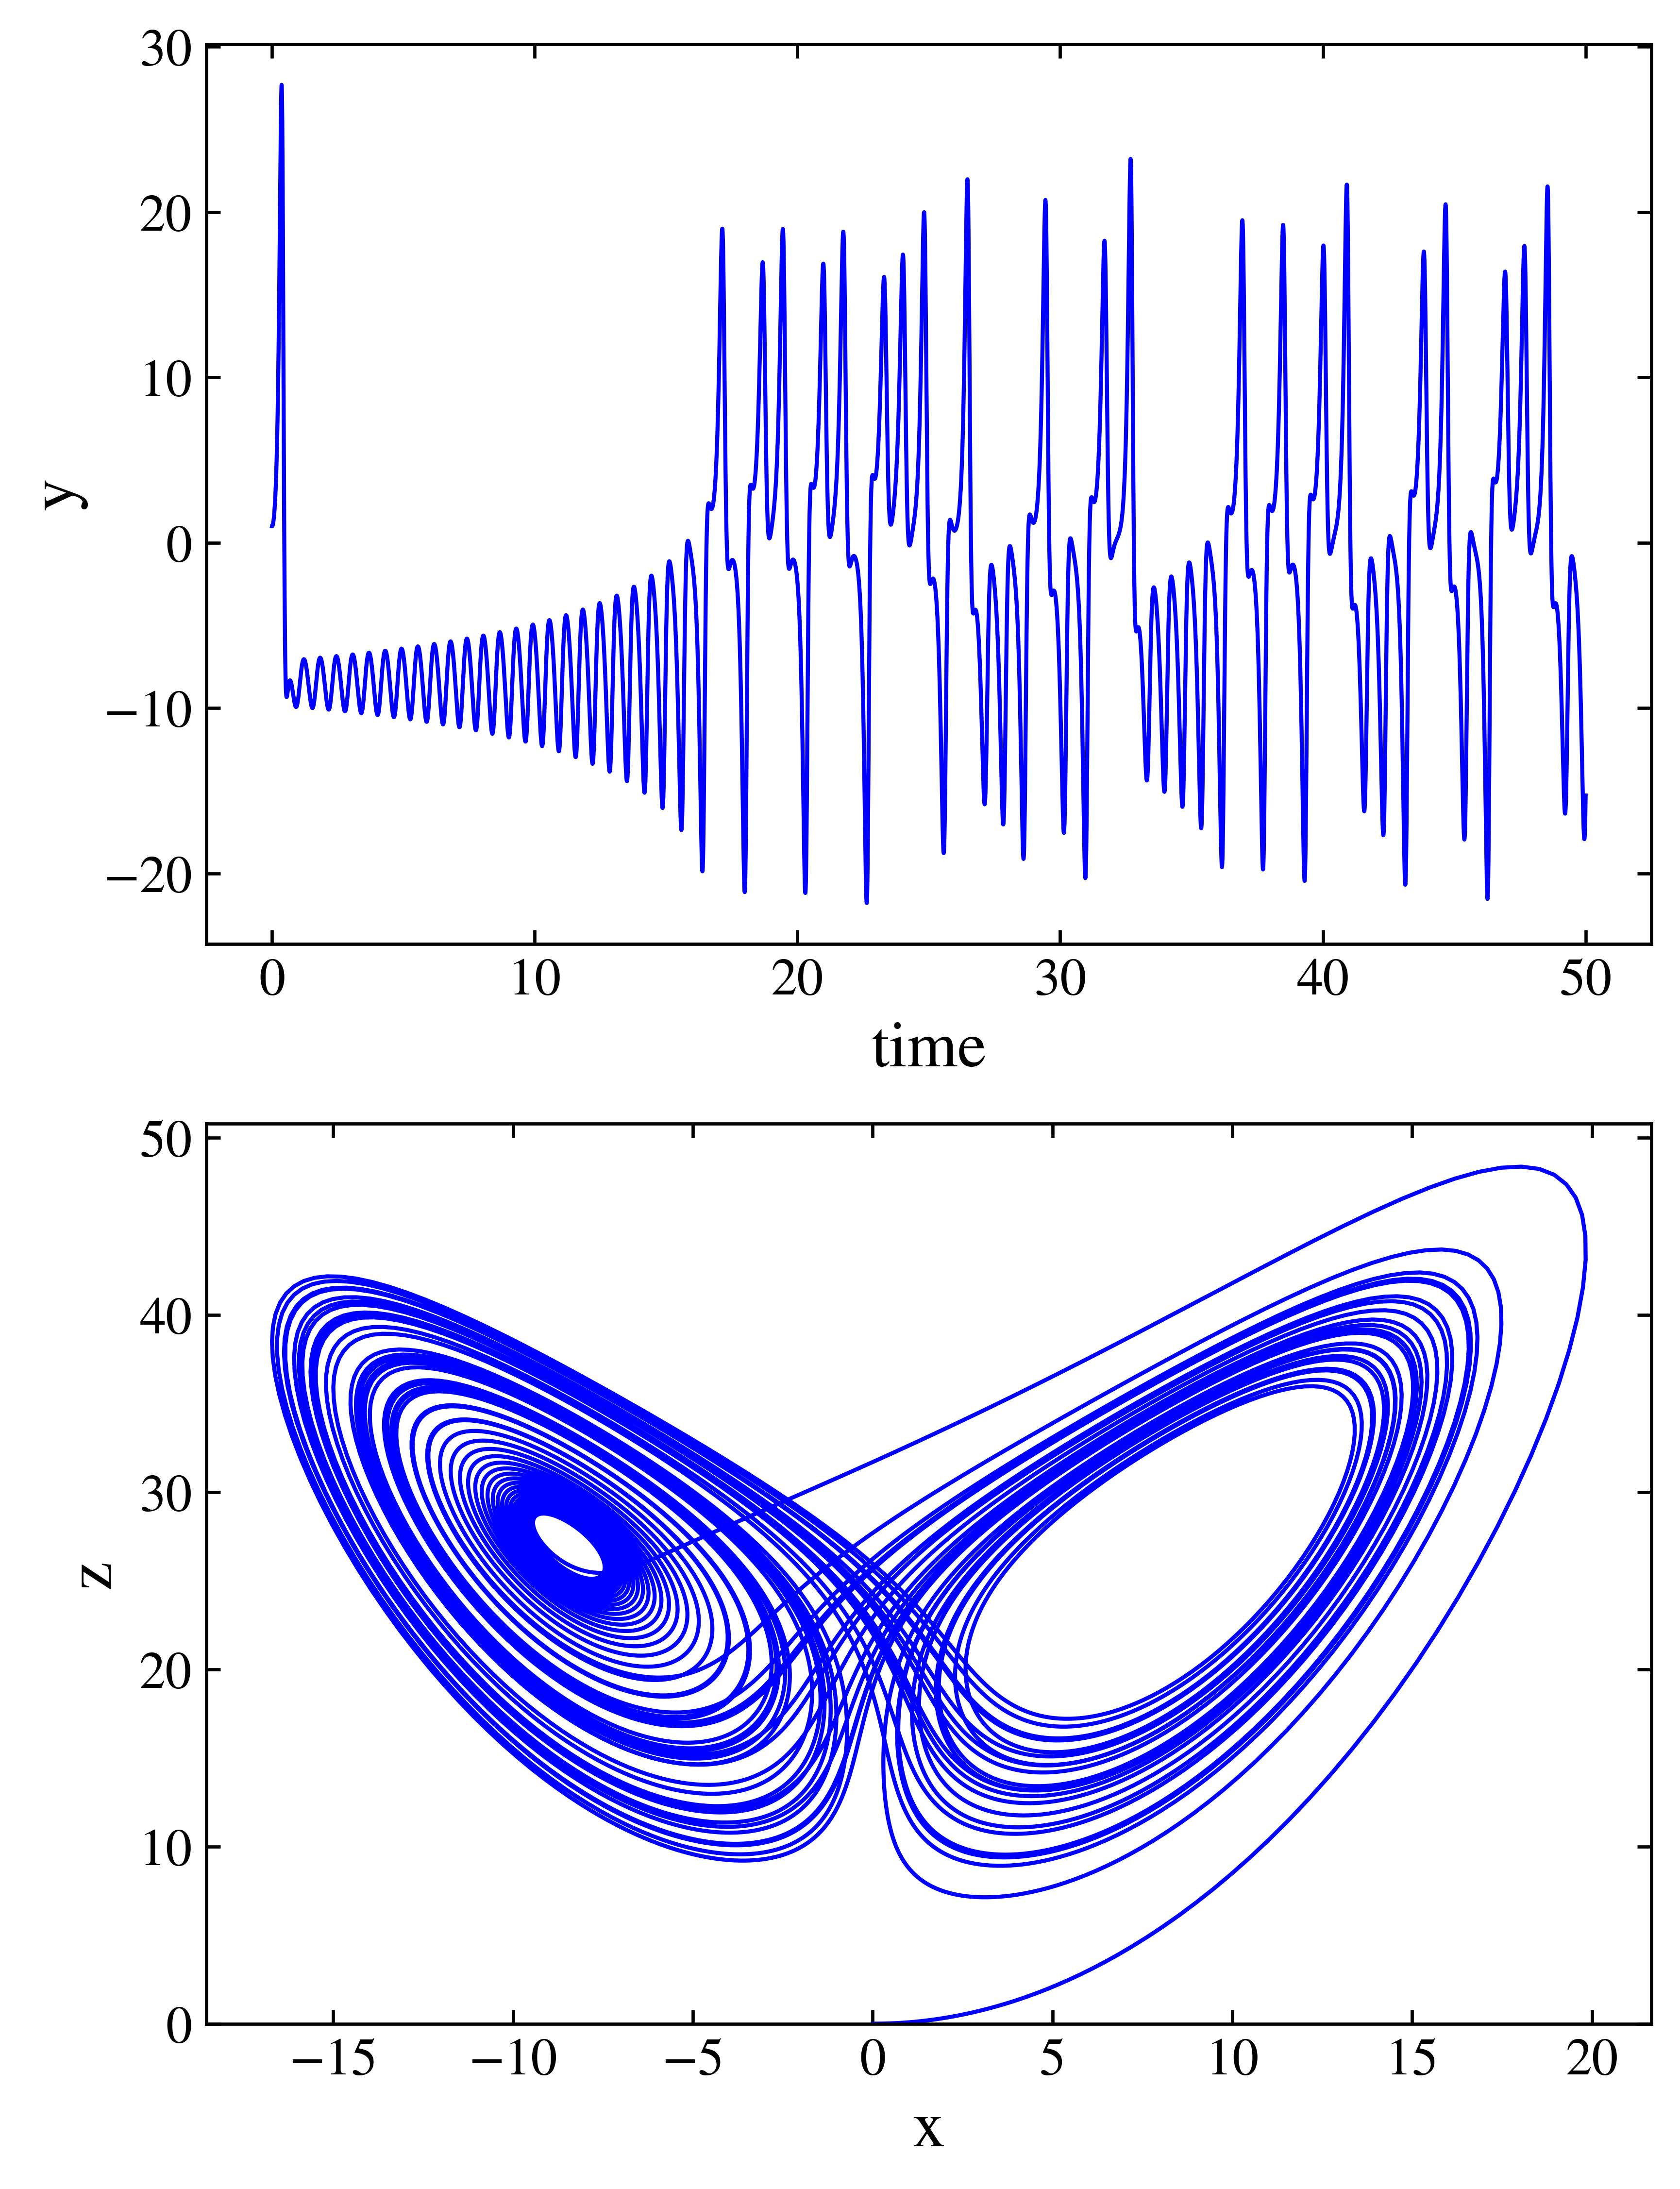
\includegraphics[width=0.48\textwidth]{fin_1}
	\caption{Behavior of Lorenz equations: (Above) y versus t, (Below) x versus z}
	\label{fig:fin1}
\end{figure}
 
\begin{enumerate}
	\item From $\sigma = 10$, $r=28$, $b = 8/3$, determine the value $y$ in range $t = 0\sim50$ from initial conditions $(x, y, z) = (0,1,0)$.
	
	To compute the Lorenz equations, I use 4th Runge-Kutta method with $N=10000$ steps until $t = 50$ s. 
\begin{Verbatim}[tabsize=3]
def RK4(f, x, t, h):
	k1 = h*f(x, t)
	k2 = h*f(x+0.5*k1, t+0.5*h)
	k3 = h*f(x+0.5*k2, t+0.5*h)
	k4 = h*f(x+k3, t+h)
	return x+ (k1+2*k2+2*k3+k4)/6.
def f(X, t):
	x,y,z = X
	fx = sigma*(y-x)
	fy = r*x - y - x*z
	fz = x*y - b*z
return np.array([fx,fy,fz])
\end{Verbatim}
	The plot of $y$ as function of $t$ shows some randomness, shown in Figure~\ref{fig:fin1}.
	
	\item Plot $z$ against $x$, which is illustrated in Figure~\ref{fig:fin1}. We can observe `strange attractor', a bitterfly-shaped spiral curve.
\end{enumerate}

\section{An electronic capacitor}
Consider model of electronic capacitor, consisting of two flat metal plates in square metal box of $100$ cm$^2$. Two $6$ cm-metal plates have fixed voltage of $\pm 1$ V seperated by $6$ cm. Moreover, the boundary of box has fixed $0$ V.

To calculate electrostatic potential in box of grid $100\times100$, I use Gauss-Seidel method with precision at each grid point of $10^{-6}$.

\begin{Verbatim}[tabsize=3]
phi = np.zeros((M, M))
phi[20:80, 20] = 1
phi[20:80, 80] = -1
d = 1.
while d>acc:
	d = 0.
	for i in range (1, M-2):
		for j in range (1, M-2):
			if j==20 or j==80:
				if i>=20 and i<80: continue
			tmp = 0.25*(phi[i+1,j] + phi[i-1,j] 
					+ phi[i,j+1] + phi[i,j-1])
			d = max(d, abs(phi[i,j]-tmp))
			phi[i,j] = tmp
\end{Verbatim}

The calculated potential values are plotted in Figure~\ref{fig:fin2}. Clearly, in the region of two line capacitors, the voltage is near $\pm 1$ V, since two plates are considered as some type of boundary conditions.

\begin{figure}[t]
	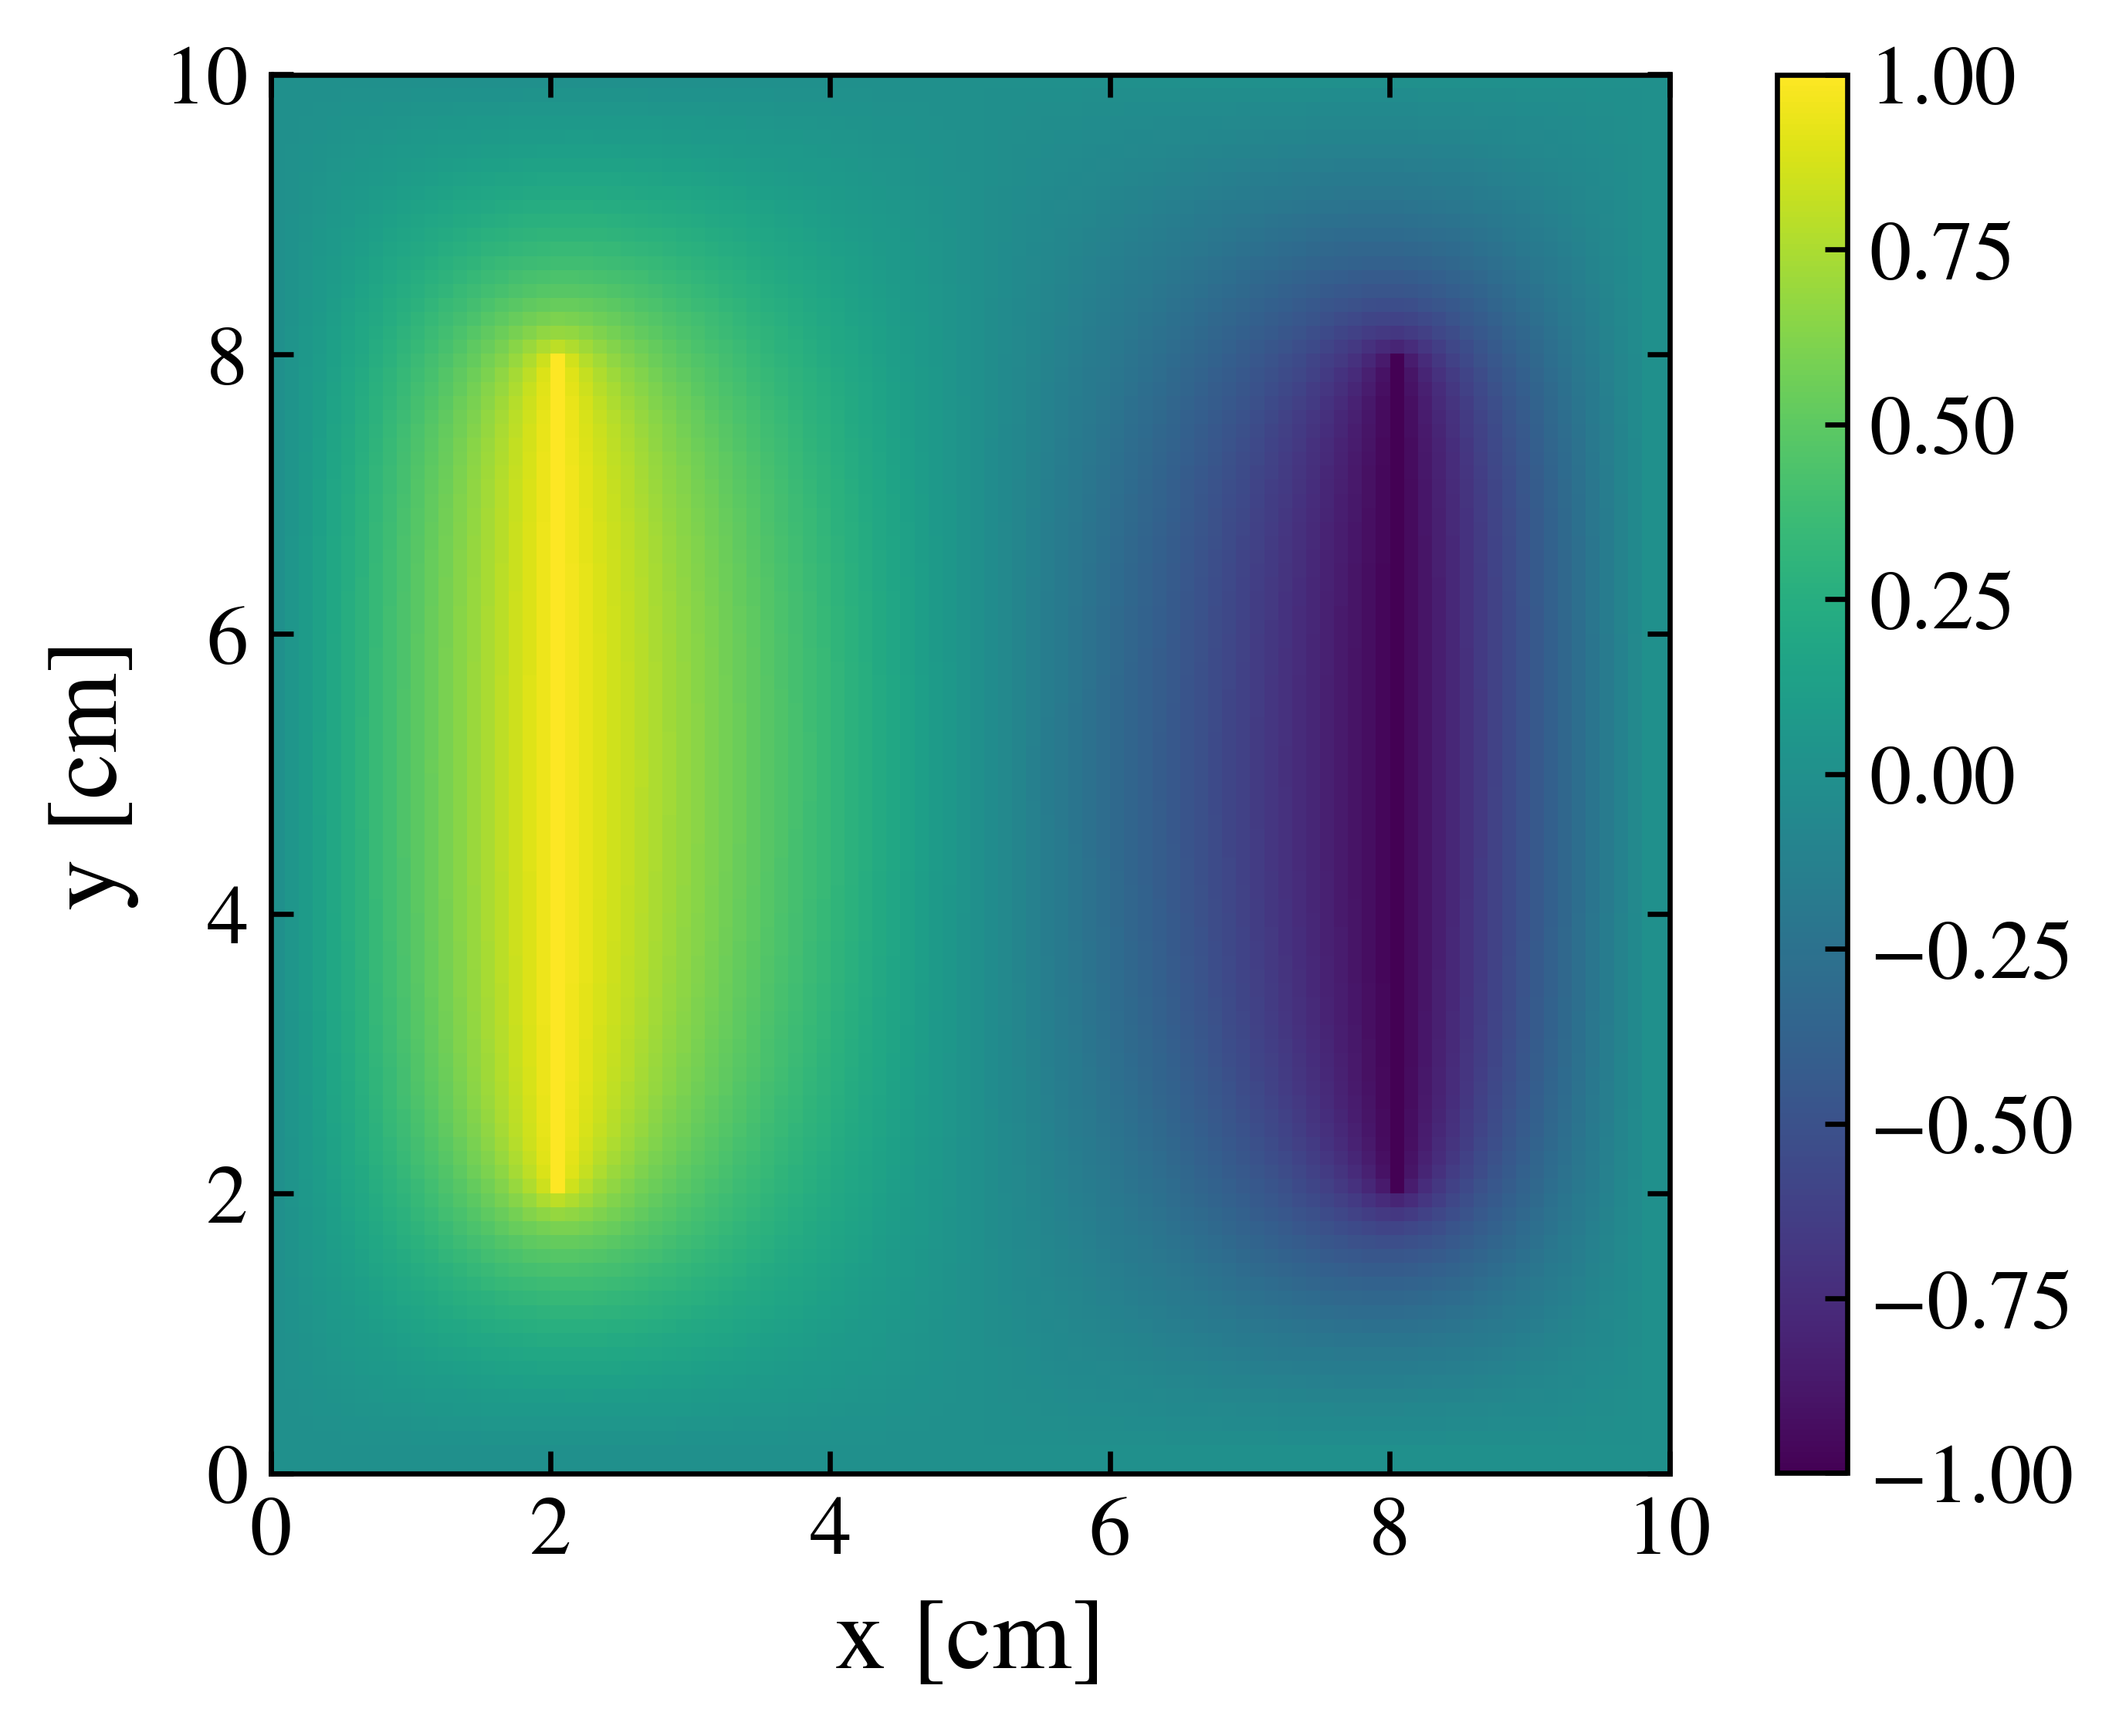
\includegraphics[width=0.45\textwidth]{fin_2}
	\caption{Plotted electrostatic potential in box with electronic capacitor.}
	\label{fig:fin2}
\end{figure}


\section{The Schr\"odinger equation and the Crank-Nocolson method}
The Schr\"odinger equation is given by
\begin{equation*}
	-\frac{\hbar^2}{2M}\frac{\pd^2\Psi}{\pd x^2} = \im\hbar \frac{\pd \Psi}{\pd t}
\end{equation*}
For particle in infinite square well of width $L$, we can obtain Crank-Nicolson equation with central time difference,
\begin{align*}
	\Psi(x, t+h) &= \Psi(x,t)\\
	&+ h\frac{\im\hbar}{4ma^2}\Bigl\{\left[\Psi(x+a, t)+\Psi(x-a, t)-2\Psi(x,t)\right]\\
	&+ \left[\Psi(x+a, t+h) + \Psi(x-a, t+h) - 2\Psi(x, t+h)\right]\Bigr\}
\end{align*}
If we rewrite the former equation with with $a = L/n$,
\begin{gather*}
	\mathbf{A} = \V{a_1&a_2\\a_2&a_1&a_2\\ &a_2&a_1 \\ &&&\ddots}\!,\; 
	\mathbf{B} = \V{b_1&b_2\\b_2&b_1&b_2\\ &b_2&b_1 \\ &&&\ddots}\\
	\psi(t) = \V{\Psi(a,t)\\\Psi(2a,t)\\\cdots\\\Psi((n-1)a,t)}\\
	\mathbf{A}\psi(t+h) = \mathbf{B}\psi(t)\\
	a_1,b_1 = 1\pm h\frac{\im\hbar}{2ma^2}, \;\,a_2,b_2 = \mp h\frac{\im\hbar}{4ma^2}
\end{gather*}
It is quite easy to reproduce this time-independent matrices.

By repeat the linear solver, one can determine the time-evolved wave function of electron which was initially
\begin{equation*}
	\Psi(x,0) = \exp\left[-\frac{(x-x_0)^2}{2\sigma^2}\right]e^{\im \kappa x}, \quad x_0 = \frac{L}{2}
\end{equation*}
where $\sigma = 10^{-10}$ m, $\kappa = 5\times 10^{10}$ m$^{-1}$.

\begin{figure}[t]
	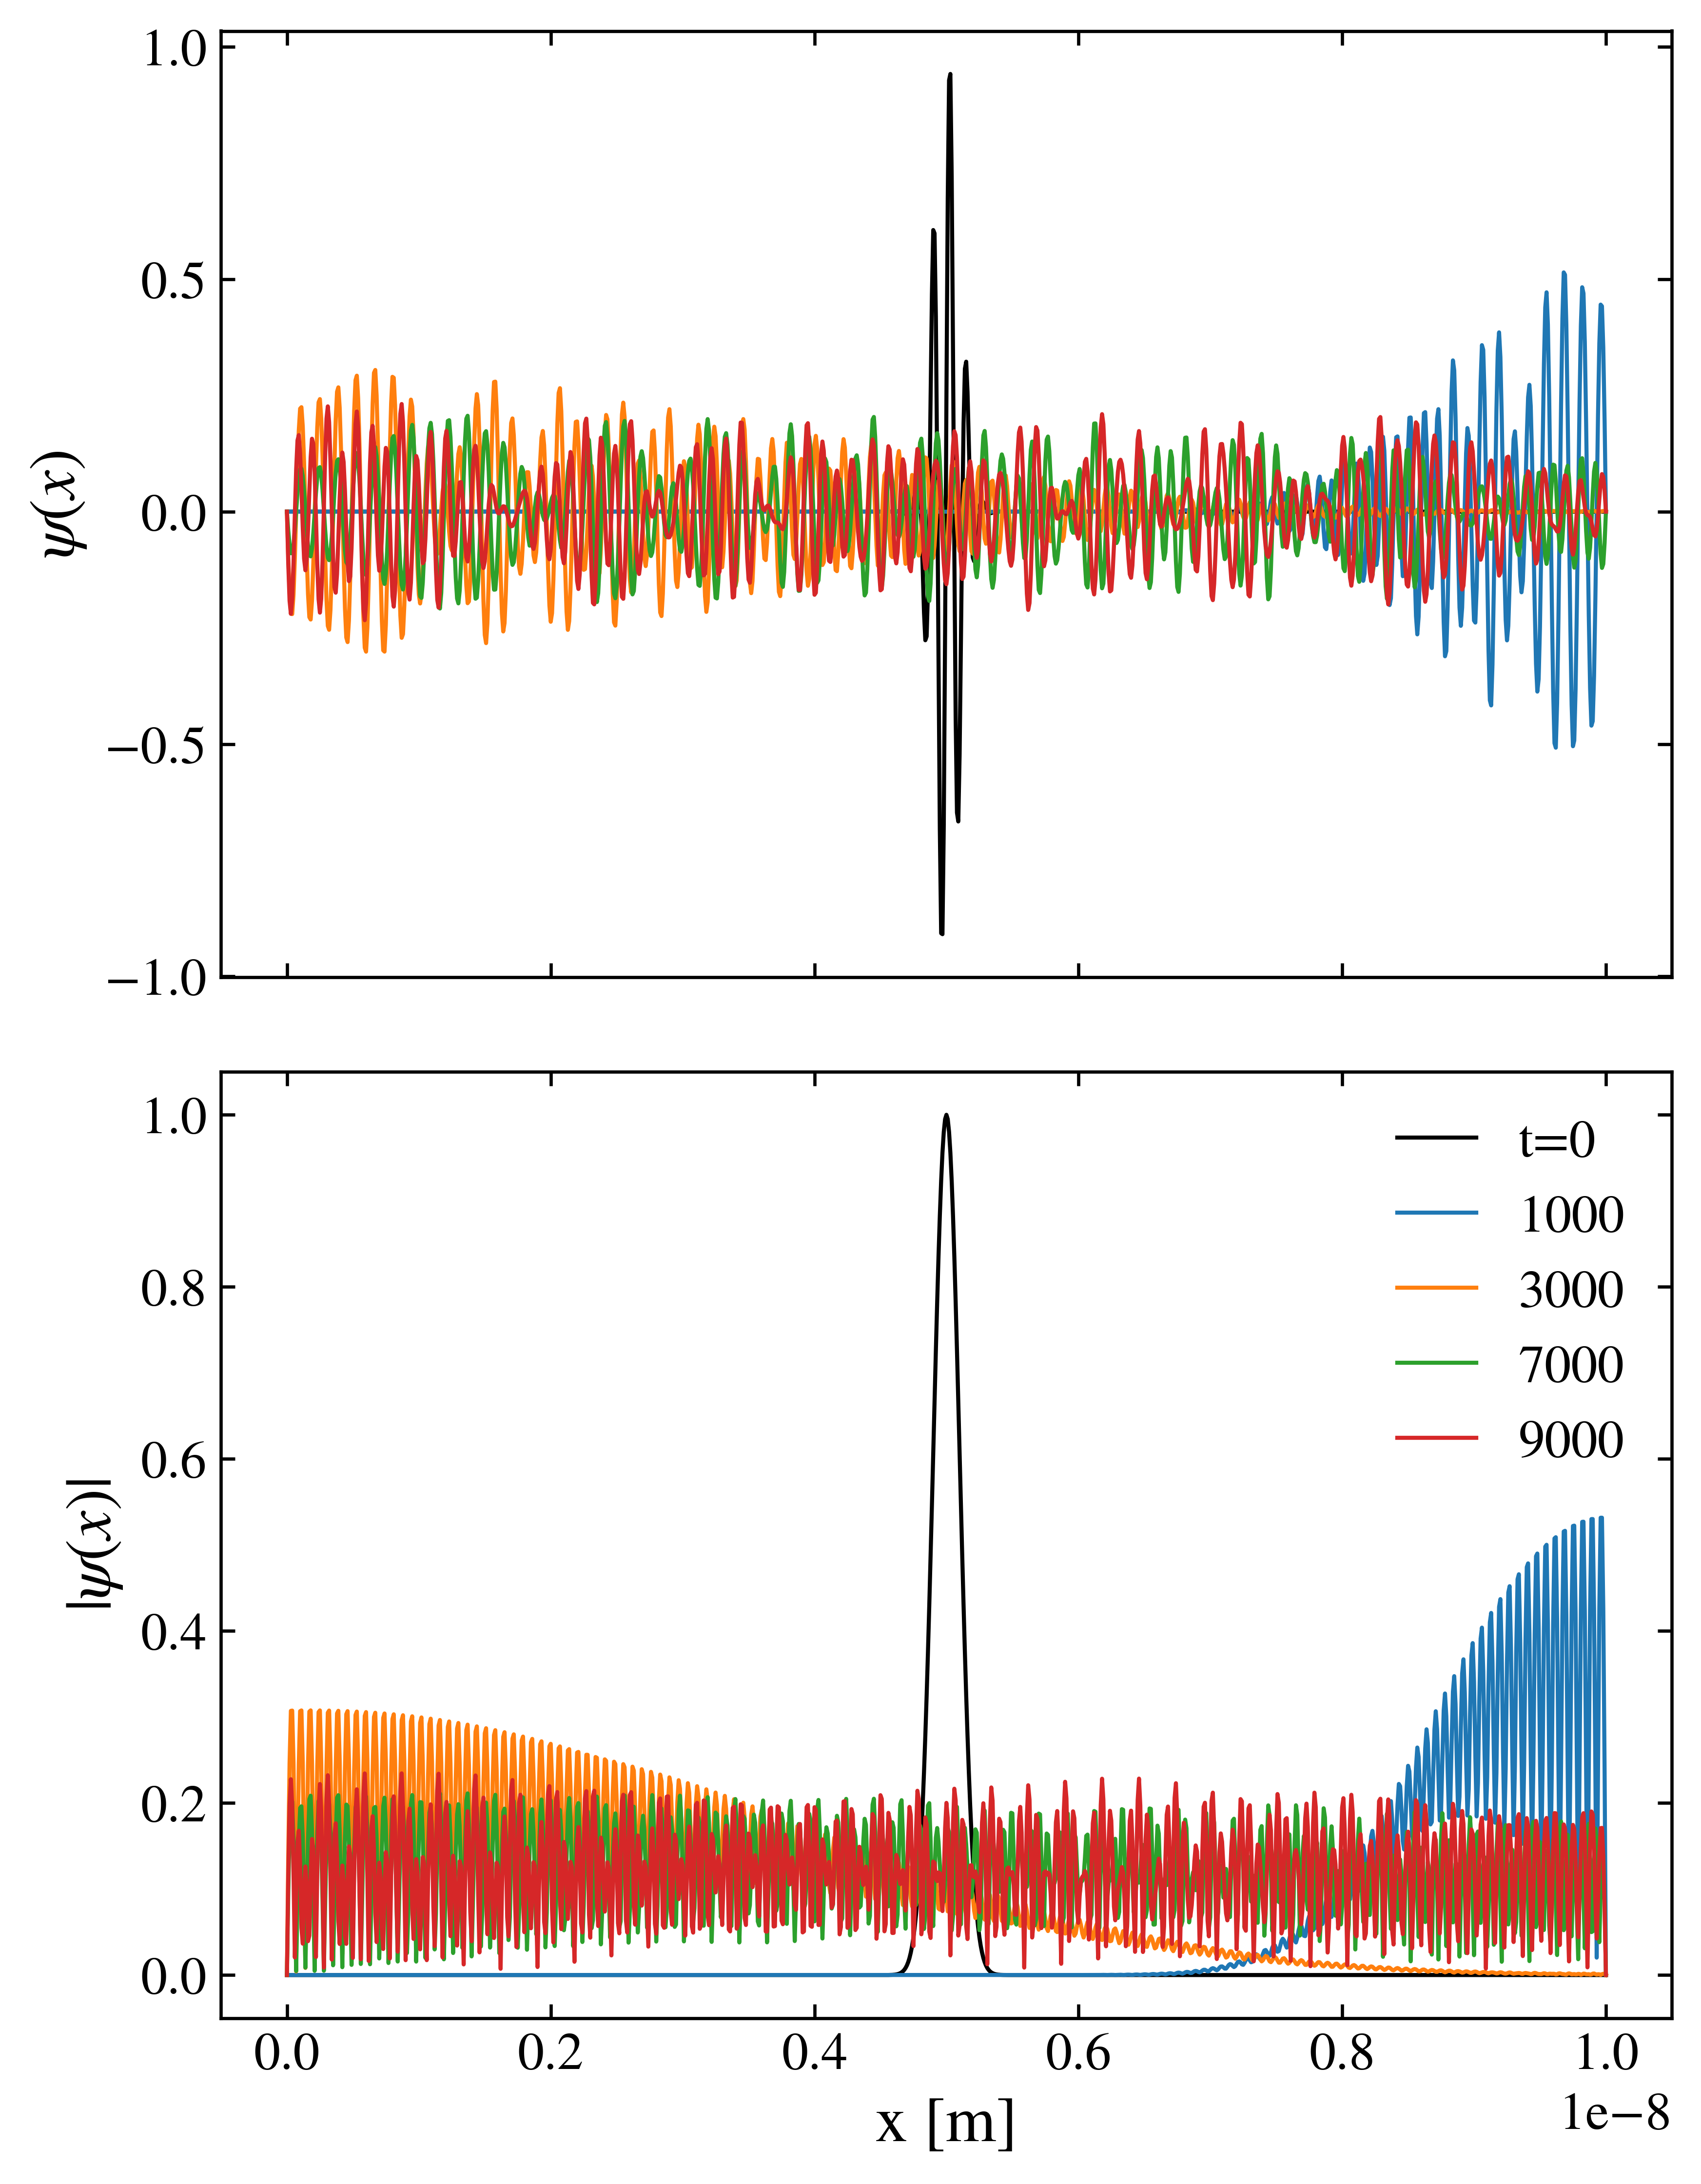
\includegraphics[width=0.48\textwidth]{fin_3}
	\caption{Wave function of electron with different time steps: (Above) real value of wave function, (Below) absolute value of wave function.}
	\label{fig:fin3}
\end{figure}

\begin{enumerate}
	\item To perform Crank-Nicolson method, I have choose time step interval $h = 10^{-18}$ and $n = 1000$ spatial slices. Also, I have performed 10000 time steps, which makes $t = 10^{-14}$ s total.

\begin{Verbatim}[tabsize = 3]
def wavef(x):
	return np.exp(-0.5j*k*x*(x-x0)**2/sigma**2)
psi = np.zeros((step,N+1), complex)
psi[0] = wavef(x)
for i in range (step-1):
	v=B.dot(psi[i,1:N])
	psi[i+1,1:N]=linalg.solve(A v,assume_a=`sym')
\end{Verbatim}

\item I have ploted real values of wave function $\Re(\Psi(t))$ and also absolute value of wave function $|\Psi(t)|$ for different time slices in Figure~\ref{fig:fin3}. For the whole time range, it is animated in \url{electron.mp4}.

\item The behavior of electron wave function:

At the first time, the electron was situated right at the center of the square well. As the time passes, it moves toward right side, and bounces back and moves toward the other side. 
As the electron is considered as wave, some fluctuations due to interference occurs when it bounces on the wall.
After large time steps, it becomes difficult to point out the position of the electron, since it is widely spreaded, with various nodes.
\end{enumerate}






%\bibliography{mid_ref}
\end{document}
